\section{Zielsetzung}
\label{sec:Zielsetzung}
Es soll die Quantennatur der Elektronenhülle von Atomen gezeigt werden. Weiterhin soll ein Zusammenhang zwischen
der Anregungsenergie und der Wellenlänge des emittierten Lichts hergestellt werden. Mit den daruas erhaltenen
Erkentnissen lassen sich die Bohrschen Postulate teilweise bestätigen. Außerdem wird die Energieverteilung der
Elektronen bestimmt.

\section{Theorie}
\label{sec:Theorie}
Es wird Hg-Dampf mit passender Dichte mit möglichst monoenergetischen Elektronen beschossen. Dabei treten
elastische und unelastische Stöße auf. Aus der Energiedifferenz der Elektronen vor und nach dem Stoß lässt
sich dann die vom Hg-Atom aufgenommene Energie bestimmen. Die unelastischen Stöße werden dabei verwendet, um
die Atome aus dem Grundzustand $E_{\symup{0}}$ in den ersten angeregten Zustand $E_{\symup{1}}$ zu heben.
Für die Energiedifferenz gilt dann
\begin{equation}
    \label{eqn:Ediff}
    \frac{m_{\symup{0}}v_{\symup{vor}}^2}{2} - \frac{m_{\symup{0}}v_{\symup{nach}}^2}{2}
    = E_{\symup{1}} - E_{\symup{0}}\,.
\end{equation}
Die Energien lassen sich mit der Gegenfeldmethode bestimmen.

\section{Aufbau und Ablauf}
\label{sec:AufbauAblauf}
In einem evakuierten Gefäß ist ein Tropfen Quecksilber, der nach der Dampfdruckkurve verdampft. Dadurch
hängt der Gleichgewichtsdampfdruck $p_{\symup{sät}}$ von der Temperatur $T$ ab. Im Gefäß wird ein Draht aus einem
hochschmelzenden Metall, wie z.B. Wolfram, mittels Gleichstrom auf Rotglut erhitzt, so dass durch den
glühelektrischen Effekt Elektronen frei werden, die sich wie eine Wolke um den Draht legen. Dieser Effekt wird
durch ein Oxid eines Erdalkalimetalls, das auf den Draht gestrichen wurde und eine geringere Austrittsarbeit
$W$ als der Draht hat, so dass mehr Elektronen frei werden. Um die Elektronen zu beschleunigen, wird eine
netzförmige Elektrode gegenüber zum Draht angebracht, an der eine Gleichspannung $U_{\symup{B}}$ zur Beschleunigung
angelegt wird. Eine schematische Darstellung des Versuchaufbaus ist in \autoref{fig:Aufbau} zu sehen.
\begin{figure}
    \centering
    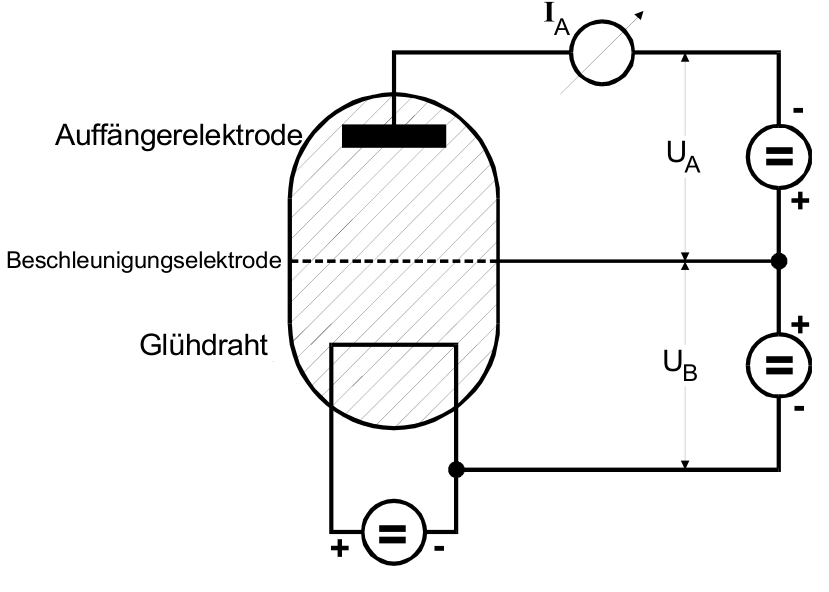
\includegraphics[width=0.7\textwidth]{Bilder/SchematischerAufbau.png}
    \caption{Schematischer Aufbau der Franck-Hertz Apparatur.}
    \label{fig:Aufbau}
\end{figure}
Nach der Beschleunigungsstrecke haben die Elektronen die Energie
\begin{equation}
    \label{eqn:E_Beschleunigung}
    \frac{m_{\symup{0}} v_{\symup{vor}}^2}{2} = \symup{e}_{\symup{0}} U_{\symup{B}}
\end{equation}
solange sie vor der Beschleunigung die Geschwindigkeit 0 hatten. Hinter der Beschleunigungselektrode befindet
sich eine Auffängerelektrode an der mit einem geeigneten Messgerät der Auffängerstrom $I_{\symup{A}}$ messbar ist.
Da die Auffängerelektrode eine geringere Spannung $U_{\symup{A}}$ als die Beschleunigungselektrode hat, müssen die
Elektronen, damit sie an der Auffängerelektrode ankommen, die Ungleichung
\begin{equation}
    \label{eqn:E_Ungleichung}
    \frac{m_{\symup{0}}}{2} v_{\symup{z}}^2 \geq \symup{e}_{\symup{0}} U_{\symup{A}}
\end{equation}
erfüllen. Im Beschleunigungsraum befinden sich nun die Hg-Atome, so dass die Elektronen mit ihnen zusammenstoßen.
Bei geringer Elektronenenergie treten nur elastische Stöße auf. Da das Massenverhältnis von Elektron und Hg-Atom
etwa $\frac{1}{1836 \cdot 201}$ beträgt, ergibt sich eine relativ geringe Energieabgabe von
\begin{equation}
    \label{eqn:EnergieAbgabe}
    \Delta E = \frac{4 m_{\symup{0}} M}{(m_{\symup{0}} + M)^2} E \approx 1,1\cdot 10^{-5} E\,.
\end{equation}
Die dabei vollzogenen Richtungsänderungen können dabei aber beträchtlich sein.